\documentclass{beamer}
\usefonttheme[onlymath]{serif}
\usepackage[english]{babel}							%For internationalization
\usepackage[utf8]{inputenc}							%For character encoding
\usepackage{amsmath}								%For mathematical typesetting
\usepackage{amssymb}								%For mathematical typesetting
\usepackage{graphicx}								%For handling graphics
\usepackage{listings}

\newcommand{\be}{\begin{equation}}
\newcommand{\ben}[1]{\begin{equation}\label{#1}}
\newcommand{\ee}{\end{equation}}
\newcommand{\aomega}{\overset{\sim}{\omega}}				%Approximate omega

\setbeamerfont{footnote}{size=\tiny}
\beamertemplatenavigationsymbolsempty
\setbeamerfont{page number in head/foot}{size=\large}
\setbeamertemplate{footline}[frame number]
\lstset{breaklines=true,basicstyle=\tiny}

\title
{In Pursuit of a Fast High-order Poisson Solver: Volume Potential Evaluation }
\author[Bevan] % (optional, for multiple authors)
{J.~Bevan, UIUC}
\institute[UIUC] % (optional)

\date[December 2017] % (optional)
{\textit{CS598 APK\\ December 8, 2017}}
\subject{Integral Equation Methods}

\begin{document}
\frame[plain,noframenumbering]{\titlepage}
\section{Introduction}
\subsection{Physical Examples and Motivating Problems} 
\frame{\frametitle{\textbf{\secname}: \subsecname}
\begin{figure}
\centering
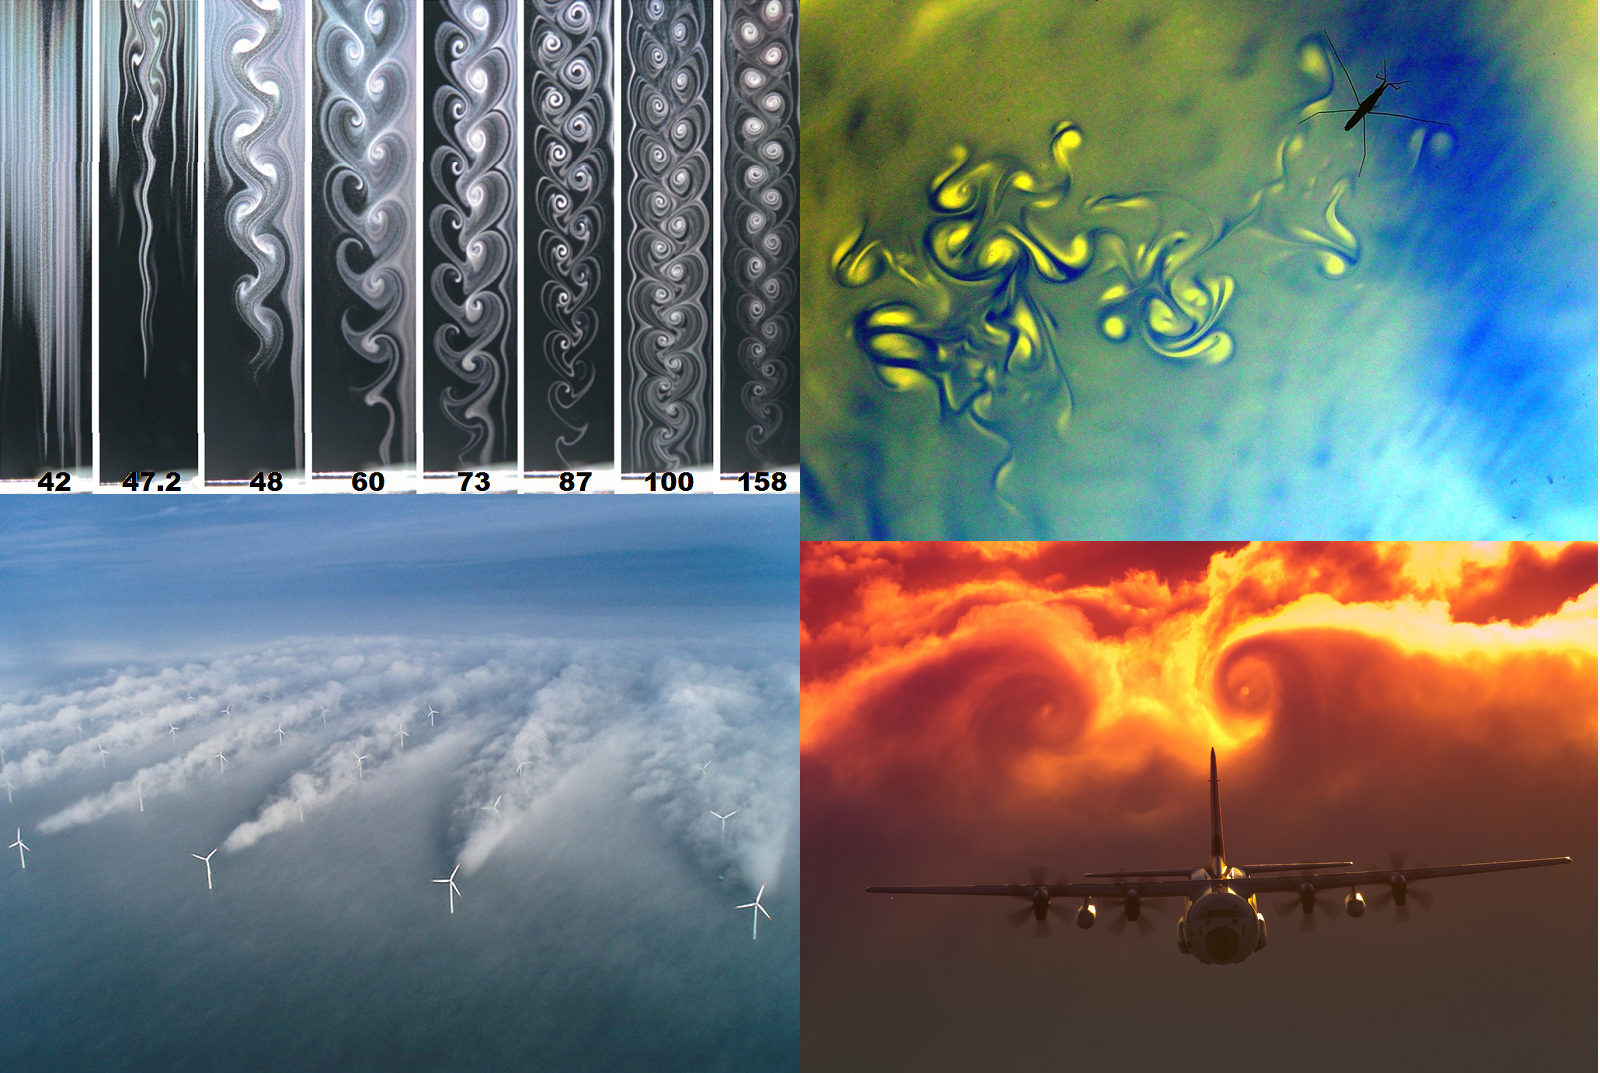
\includegraphics[width=4.5in]{Composite.PNG}
\end{figure}
}

\subsection{What is Vorticity?} 
\frame{\frametitle{\subsecname}
\be \mathbf{\omega} = \nabla \times \mathbf{u} \ee

\be \Gamma = \oint_{\partial S}\mathbf{u}\cdot \,d\mathbf{l}= \int\!\!\!\int_S \omega \cdot \,d\mathbf{S} \ee
\begin{figure}
\centering
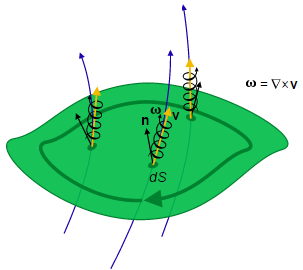
\includegraphics[width=2in]{VortDiag.PNG}
\end{figure}

\footnotetext{https://commons.wikimedia.org/wiki/File:Generalcirculation-vorticitydiagram.svg}
}

\subsection{Some Brief Theory} 
\frame{\frametitle{\subsecname}
Navier-Stokes momentum equation
 \be \rho \left(\frac{\partial \mathbf{u}}{\partial t} + \mathbf{u} \cdot \nabla \mathbf{u} \right) = -\nabla p + \mu \nabla^2 \mathbf u + \tfrac13 \, \mu \nabla (\nabla\cdot\mathbf{u}) \ee
where $u$ is the velocity field, $p$ is the pressure field, and $\rho$ is the density.
Navier-Stokes can be recast as
\ben{VV3D} \frac{\partial \omega}{\partial t} +  \mathbf{u} \cdot \nabla \omega - \omega \cdot \nabla  \mathbf{u} = S(x,t)\ee
 viscous generation of vorticity, $S$
 For incompressible flows velocity related to vorticity by
\be \nabla^2 \mathbf{u} = -\nabla \times \omega \ee
Invert to obtain Biot-Savart integral
\ben{BS} \mathbf{u}(x) = \int_\Omega K(x,y) \times \omega(y) dx \ee
$x$ is velocity eval point, $y$ is non-zero vorticity domain, $K(x,y)$ singular Biot-Savart kernel.
}

\subsection{Why Integral Equation Methods?} 
\frame{\frametitle{\subsecname}
\begin{itemize}
\item Low-order solvers common (for both Lagrangian\footnotemark\, and Eulerian\footnotemark \, approaches)
\item Some ``high''-order work exists\footnotemark, but is special purpose
\item Ultimately, choice must be made between what form of Poisson equation is most useful
\item Integral equations offer robust and flexible way, especially for complex geometries and for high-order
\end{itemize}

\footnotetext[1]{Moussa, C., Carley, M. J. (2008). A Lagrangian vortex method for unbounded flows. International journal for numerical methods in fluids, 58(2), 161-181.}
\footnotetext[2]{R.E. Brown. Rotor Wake Modeling for Flight Dynamic Simulation of Helicopters. AIAA Journal, 2000. Vol. 38(No. 1): p. 57-63.}
\footnotetext[3]{J. Strain. Fast adaptive 2D vortex methods. Journal of computational physics 132.1 (1997): 108-122.}
\footnotetext[4]{Gholami, Amir, et al. "FFT, FMM, or Multigrid? A comparative Study of State-Of-the-Art Poisson Solvers for Uniform and Nonuniform Grids in the Unit Cube." SIAM Journal on Scientific Computing 38.3 (2016): C280-C306.}
}

\section{Methodology}
\subsection{Evaluation approach} 
\frame{\frametitle{\textbf{\secname}: \subsecname}
\begin{itemize}
\item Volume potential share similarities to layer potentials
\item Same main challenge: devising quadrature to handle singularity
\item Take same approach: QBX
\item But where do we put our expansion center, fictitious dimension?
\item Off-surface: layer potential physically defined, off-volume has no requirements
\end{itemize}
\begin{figure}
\centering
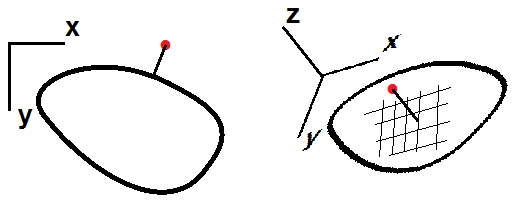
\includegraphics[width=4in]{LayVol.PNG}
\end{figure}
}

\subsection{Trial Scheme} 
\frame{\frametitle{\subsecname}
\begin{itemize}
\item Absent any compelling choice for off-volume potential, choose obvious one:
\item Consider 3D Poisson scheme: approximate $1/r$ kernel with $1/(r^2+a^2)^{1/2}$
\item Effectively $a$ parameter is the distance from expansion center to eval point in the fictitious dimension, and kernel is no longer singular
\item Choose a ``good'' $a$ so the kernel is smooth and take QBX approach of evaluating Taylor expansion of de-singularized kernel back at desired eval point
\end{itemize} 
}

\subsection{Is trial scheme high-order?} 
\frame{\frametitle{\subsecname}
\begin{itemize}
\item No, in fact seems to be limited to second order regardless of expansion order.
\item Consider example results in figure below for 5th order expansion.
\item Why only second order?
\end{itemize}
\begin{figure}
\centering
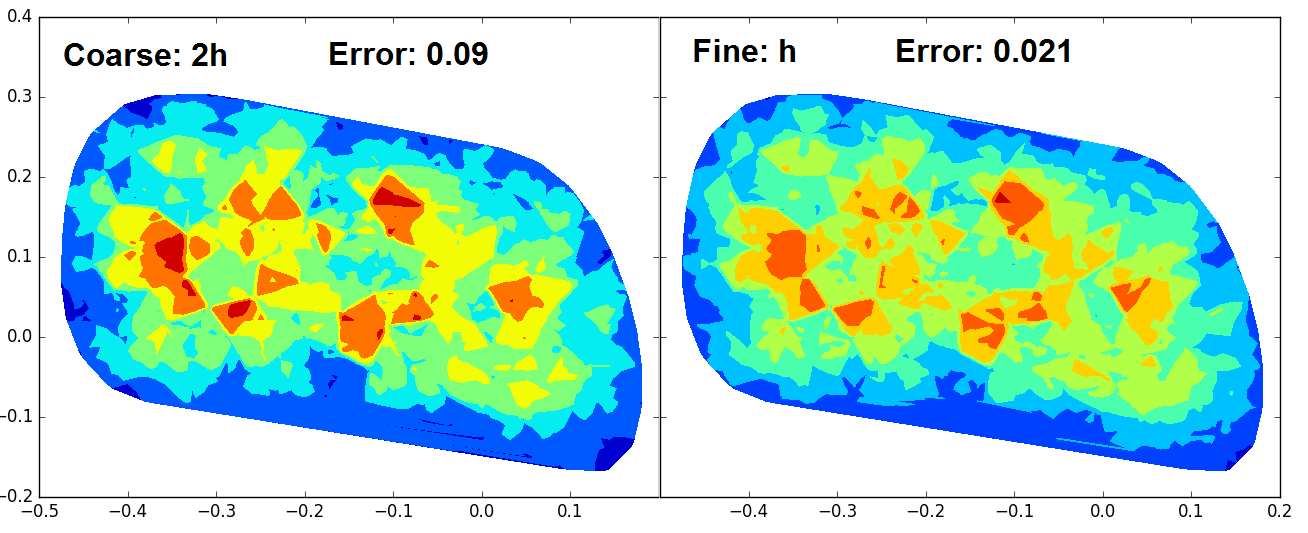
\includegraphics[width=4in]{coarseFINE.PNG}
\end{figure}
}

\subsection{Preliminary Error Analysis} 
\frame{\frametitle{\subsecname}
\begin{itemize}
\item We would like to examine the error
\item 
\item 
\end{itemize} 
}

\subsection{PH} 
\frame{\frametitle{\subsecname}
PH
\begin{itemize}
\item 
\item 
\item 
\end{itemize} 
}

\end{document}